\documentclass[letterpaper,10pt]{article}
\usepackage[letterpaper,margin=0.75in]{geometry}
\usepackage[T1]{fontenc}
\usepackage{times}
\usepackage{amsmath,amssymb,bm,graphicx,float,booktabs,array}
\usepackage{xcolor,enumitem,tcolorbox,listings,textcomp,empheq}
\usepackage[hidelinks]{hyperref}
\setlength{\parindent}{0pt}
\setlength{\parskip}{5pt}
\setlist[enumerate]{itemsep=0.6em,topsep=0.4em}
\lstdefinestyle{mymatlab}{language=Matlab,
 basicstyle=\ttfamily\footnotesize,keywordstyle=\color{blue!70!black},
 stringstyle=\color{teal!60!black},commentstyle=\itshape\color{gray!70},
 emph={t1,y1,G1,num1,den1},emphstyle=\color{magenta}\bfseries,
 numbers=left,numberstyle=\tiny\color{gray!70},backgroundcolor=\color{gray!5},
 frame=single,showstringspaces=false,upquote=true,breaklines=true,
 columns=fullflexible,keepspaces=true,xleftmargin=1.5em,framexleftmargin=0.3em}
\lstset{style=mymatlab}
\newcommand{\RMS}{\mathrm{RMS}}
\newcommand{\dd}{\,\mathrm{d}}
\newcommand{\dochead}[1]{\begin{center}{\Large\bfseries ME 4030: Final Project}\\[5pt]
 {\large #1}\\[4pt]Quarter-Car Active Suspension\\
 Corrected public edition, September 2026\end{center}}
\newcommand{\task}[1]{\subsection*{#1}}
\newcommand{\eom}{\begin{align}
 M_s\ddot z_s&=-K_s(z_s-z_u)-C_s(\dot z_s-\dot z_u)+u,\label{eq:body}\\
 M_u\ddot z_u&=K_s(z_s-z_u)+C_s(\dot z_s-\dot z_u)-K_t(z_u-z_r)-C_t(\dot z_u-\dot z_r)-u.\label{eq:wheel}
 \end{align}}
\newcommand{\parameters}{\begin{center}\begin{tabular}{lll}\toprule
 Parameter & Value & Meaning\\\midrule
 $M_s$ & $2500\ \mathrm{kg}$ & Sprung mass\\
 $M_u$ & $320\ \mathrm{kg}$ & Unsprung mass\\
 $K_s$ & $80000\ \mathrm{N/m}$ & Suspension stiffness\\
 $C_s$ & $350\ \mathrm{N\,s/m}$ & Suspension damping\\
 $K_t$ & $500000\ \mathrm{N/m}$ & Tire stiffness\\
 $C_t$ & $15020\ \mathrm{N\,s/m}$ & Tire damping\\\bottomrule
 \end{tabular}\end{center}}

\begin{document}
\dochead{Worked Solutions}
\textbf{Scope.} This is a worked reference design for the corrected project handout,
not a claim that all benchmarks can be met with one tuning. Equations, gains, plots,
and tables use the same MATLAB model and \texttt{solutions/config.json}.
The original project diagram is retained; controller plots are regenerated from
the corrected MATLAB implementation. Historical plots are not used as numerical evidence.
\begin{figure}[H]\centering
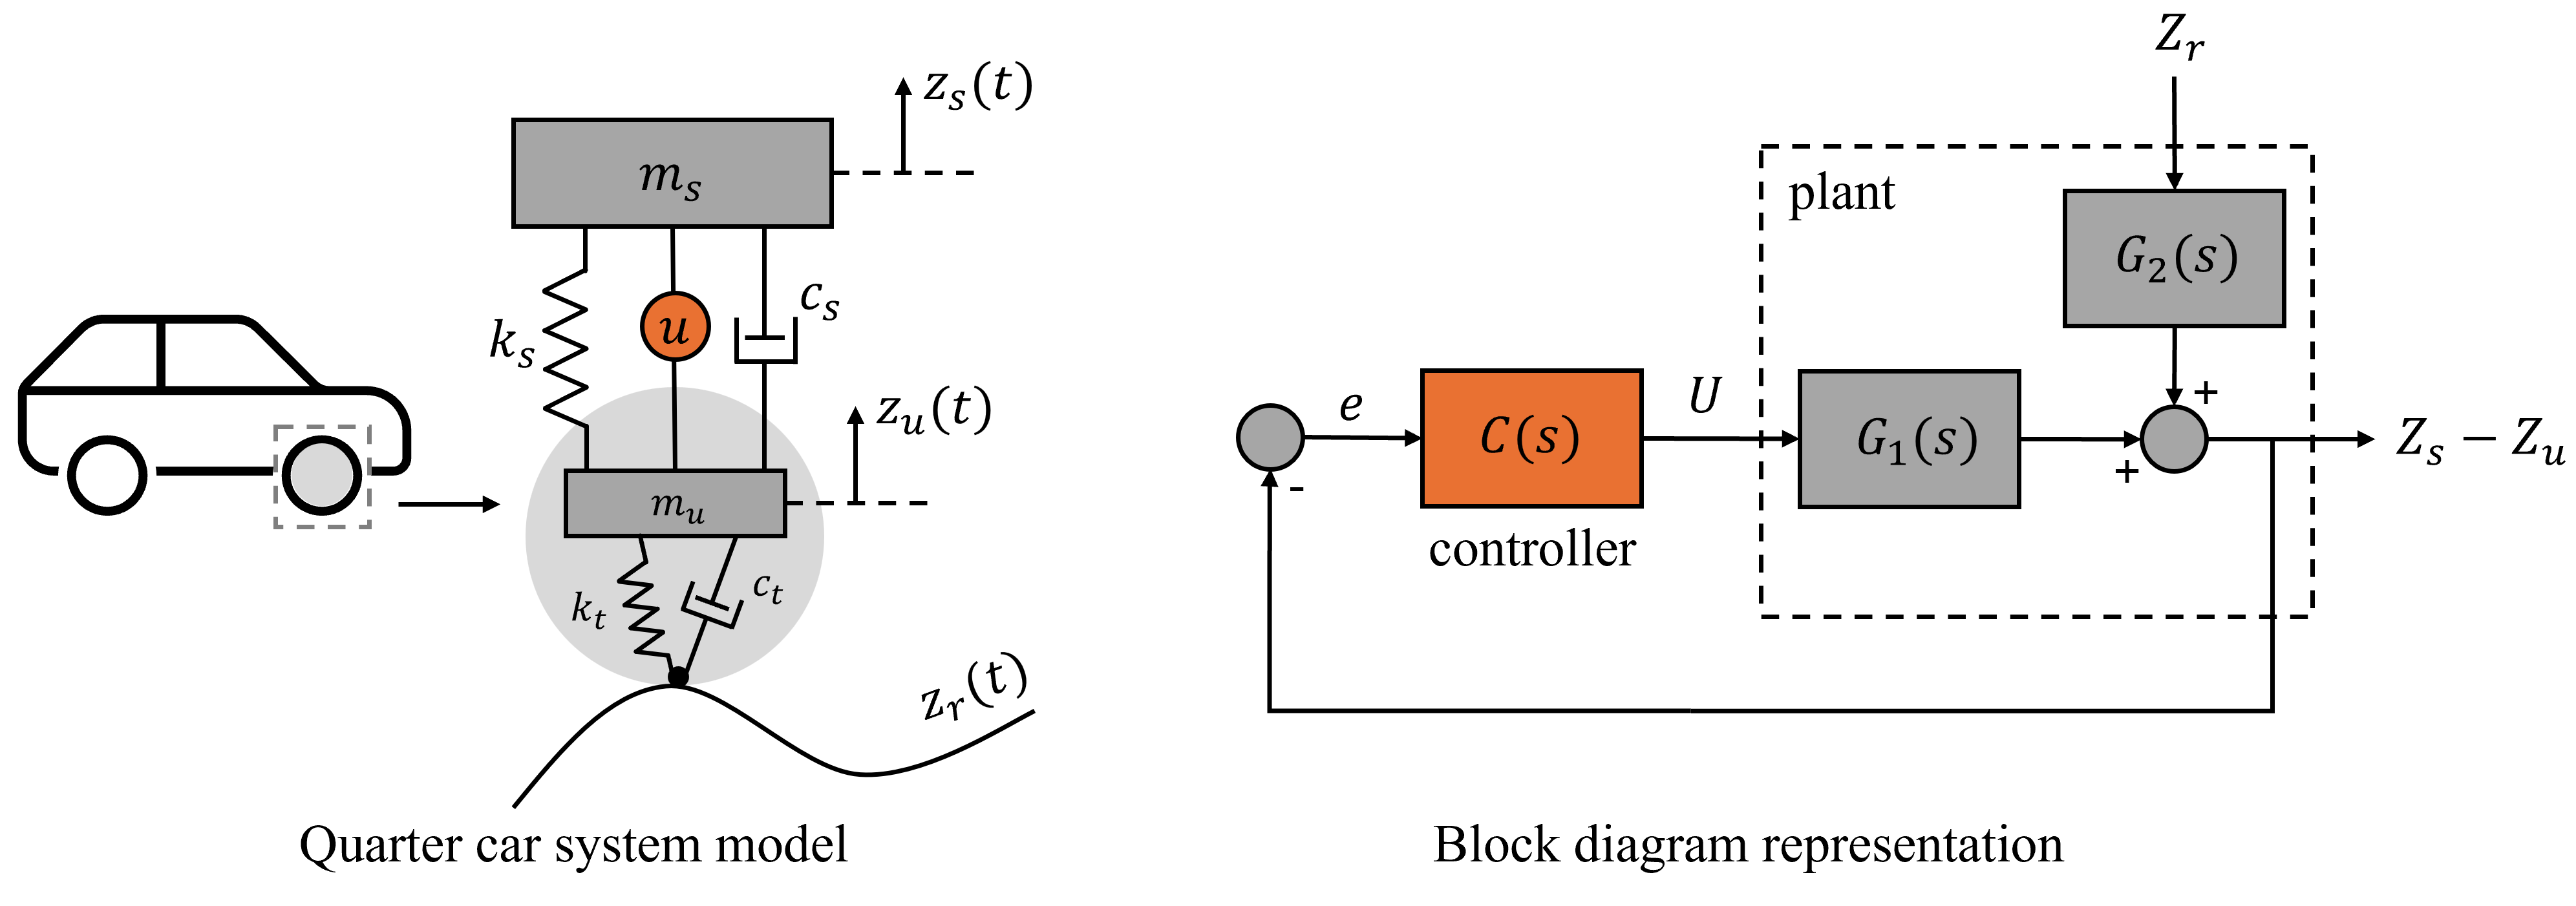
\includegraphics[width=0.58\linewidth,height=2.3in,keepaspectratio]{figures/ME4030_project.png}
\caption{Original quarter-car diagram supplied with the project.}
\end{figure}
\parameters
\section*{Model conventions}
All displacements are perturbations about static equilibrium with one common
positive direction. Let $x_s=z_s-z_u$ and $x_h=z_u-z_r$. The actuator exerts equal
and opposite forces. Newton's law gives
\eom
Positive tire deflection and its derivative create restoring terms on the wheel.
Reversing the suspension output sign requires reversing the feedback convention;
mixing the two definitions is an error.
\newpage
\task{Task 1(a,b): Transfer functions}
With zero initial conditions and Laplace variable $p$, define
\begin{align}
 a(p)&=M_sp^2+C_sp+K_s,&b(p)&=C_sp+K_s,\\
 d(p)&=M_up^2+(C_s+C_t)p+K_s+K_t,&e(p)&=C_tp+K_t.
\end{align}
The transformed force balances are
\begin{equation}
 \begin{bmatrix}a&-b\\-b&d\end{bmatrix}
 \begin{bmatrix}Z_s\\Z_u\end{bmatrix}
 =\begin{bmatrix}1&0\\-1&e\end{bmatrix}\begin{bmatrix}U\\Z_r\end{bmatrix}.
\end{equation}
The inverse of the dynamic-stiffness matrix is \emph{not} itself the input/output
transfer matrix. First invert, then multiply by the input-force matrix:
\begin{align}
 \Delta(p)&=a(p)d(p)-b(p)^2,\\
 \begin{bmatrix}Z_s\\Z_u\end{bmatrix}
 &=\frac1\Delta\begin{bmatrix}d&b\\b&a\end{bmatrix}
 \begin{bmatrix}1&0\\-1&e\end{bmatrix}\begin{bmatrix}U\\Z_r\end{bmatrix}
 =\frac1\Delta\begin{bmatrix}d-b&be\\b-a&ae\end{bmatrix}\begin{bmatrix}U\\Z_r\end{bmatrix}.
\end{align}
Subtract the second output from the first:
\begin{empheq}[box=\fbox]{align}
 G_1(p)=\frac{X_s}{U}\bigg|_{Z_r=0}&=\frac{(M_s+M_u)p^2+C_tp+K_t}{\Delta(p)},\\
 G_2(p)=\frac{X_s}{Z_r}\bigg|_{U=0}&=\frac{-M_sp^2(C_tp+K_t)}{\Delta(p)}.
\end{empheq}
Expansion gives
\begin{align}
\Delta(p)={}&M_sM_up^4+[M_s(C_s+C_t)+M_uC_s]p^3\nonumber\\
 &+[M_s(K_s+K_t)+M_uK_s+C_sC_t]p^2\nonumber\\
 &+(C_sK_t+C_tK_s)p+K_sK_t,\\
\Delta(p)={}&800000p^4+38537000p^3+1480857000p^2
 +1376600000p+40000000000,\\
G_1(p)={}&\frac{2820p^2+15020p+500000}{\Delta(p)},\qquad
G_2(p)=\frac{-37550000p^3-1250000000p^2}{\Delta(p)}.
\end{align}
Checks: $G_1(0)=1/K_s$ (static actuator force stretches the suspension),
$G_2(0)=0$ (both masses eventually follow a constant road height), and both
transfer functions are strictly proper.
\task{Task 1(c): Passive response}
Set $u=0$ and use $X_s=G_2Z_r$. For the delayed step,
$Z_r(p)=0.20e^{-p}/p$; for the sine, $Z_r(p)=0.10\pi/(p^2+\pi^2)$.
Recover body and wheel motion from $be/\Delta$ and $ae/\Delta$, respectively.
The physical four-state poles are
\begin{equation}
 -23.975782\pm35.186924\mathrm{i},\qquad -0.109843\pm5.250445\mathrm{i}.
\end{equation}
All real parts are negative, but the lightly damped body mode explains the
long passive oscillation. Its step response does not settle during the 10 s record.
\newpage
\task{Task 1(d): PID design and disturbance feedback}
Use reference $r=0$, error $e_c=r-x_s=-x_s$, and
\begin{align}
 \dot\xi&=x_s,&u&=-K_px_s-K_d\dot x_s-K_i\xi,\\
 C_{\mathrm{PID}}(p)&=K_p+K_dp+K_i/p.
\end{align}
Since $X_s=G_1U+G_2Z_r$ and $U=-C_{\mathrm{PID}}X_s$,
\begin{empheq}[box=\fbox]{align}
 \frac{X_s}{Z_r}&=\frac{G_2}{1+G_1C_{\mathrm{PID}}},&
 \frac{U}{Z_r}&=\frac{-C_{\mathrm{PID}}G_2}{1+G_1C_{\mathrm{PID}}}.
\end{empheq}
This differs from the reference-tracking transfer function
$G_1C_{\mathrm{PID}}/(1+G_1C_{\mathrm{PID}})$ displayed during tuning.
Write $N_1=(M_s+M_u)p^2+C_tp+K_t$ and $N_2=-M_sp^2(C_tp+K_t)$.
Then the disturbance response has denominator
\begin{equation}
 D_c(p)=p\Delta(p)+(K_dp^2+K_pp+K_i)N_1(p),\qquad
 \frac{X_s}{Z_r}=\frac{pN_2(p)}{D_c(p)}.
\end{equation}
Retaining the supplied example PID gains gives
\begin{equation}
 K_p=208000\ \mathrm{N/m},\quad
 K_d=832000\ \mathrm{N\,s/m},\quad
 K_i=624000\ \mathrm{N/(m\,s)}.
\end{equation}
These are an illustrative ideal-derivative design, not a feasible actuator specification.
Its poles are approximately
\begin{equation}
 -2974.911350,\quad -2.857898\pm12.904228\mathrm{i},\quad
 -0.172052\pm0.849037\mathrm{i}.
\end{equation}
The response is asymptotically stable; the fastest mode has a $0.336$ ms time constant.
A 1 ms output grid alone is inadequate for a trapezoidal force-energy integral.
\task{Task 1(e,f): Step and sine interpretation}
The integral of the wheel equation across an ideal step of height $h$ yields
\begin{equation}
 \Delta\dot z_u=\frac{C_t}{M_u}h=9.3875\ \mathrm{m/s},\qquad
 \Delta\dot z_s=0,\qquad \Delta\dot x_s=-9.3875\ \mathrm{m/s}.
\end{equation}
Positions and $\xi$ stay continuous. The derivative feedback therefore produces
\begin{equation}
 u(1^+)=K_d\frac{C_t}{M_u}h=7{,}810{,}400\ \mathrm{N}.
\end{equation}
This finite jump is extreme; it is not an impulse in actuator force. The road
derivative is impulsive because the road displacement is discontinuous.
The PID keeps suspension travel small by forcing the body to follow the wheel,
at the expense of body acceleration and force. The smooth sine avoids this step
jump, but the same tuning still misses the acceleration benchmark. Numerical
tables and corrected MATLAB plots follow after the LQR derivation.
\newpage
\task{Task 2(a): Physical state-space model}
Let $q=[z_s,\dot z_s,z_u,\dot z_u]^T$. Rearranging the two force balances gives
\begin{align}
 \dot q&=\bar A q+B_u u+B_{z_r}z_r+B_{\dot z_r}\dot z_r,\\
 \bar A&=\begin{bmatrix}
 0&1&0&0\\-K_s/M_s&-C_s/M_s&K_s/M_s&C_s/M_s\\
 0&0&0&1\\K_s/M_u&C_s/M_u&-(K_s+K_t)/M_u&-(C_s+C_t)/M_u
 \end{bmatrix},\\
 B_u&=\begin{bmatrix}0\\1/M_s\\0\\-1/M_u\end{bmatrix},\quad
 B_{z_r}=\begin{bmatrix}0\\0\\0\\K_t/M_u\end{bmatrix},\quad
 B_{\dot z_r}=\begin{bmatrix}0\\0\\0\\C_t/M_u\end{bmatrix},\qquad
 x_s=\begin{bmatrix}1&0&-1&0\end{bmatrix}q.
\end{align}
\task{Task 2(b): Eliminate the road derivative}
Define
\begin{equation}
 \alpha=\frac{C_s}{M_s}+\frac{C_s+C_t}{M_u},\quad
 \beta=\frac{K_s}{M_s}+\frac{K_s+K_t}{M_u},\quad
 \gamma=\frac1{M_s}+\frac1{M_u}.
\end{equation}
Subtracting wheel acceleration from body acceleration and using
$z_u=z_s-x_s$, $\dot z_u=\dot z_s-\dot x_s$, gives
\begin{equation}
 \ddot x_s=-\beta x_s-\alpha\dot x_s+\frac{K_t}{M_u}z_s
 +\frac{C_t}{M_u}\dot z_s+\gamma u-\frac{K_t}{M_u}z_r-\frac{C_t}{M_u}\dot z_r.
\end{equation}
Choose a velocity-like coordinate
\begin{align}
 \eta&=\dot x_s-\frac{C_t}{M_u}z_s+\alpha x_s+\frac{C_t}{M_u}z_r,\\
 \dot\eta&=\ddot x_s-\frac{C_t}{M_u}\dot z_s+\alpha\dot x_s+\frac{C_t}{M_u}\dot z_r
 =\frac{K_t}{M_u}z_s-\beta x_s+\gamma u-\frac{K_t}{M_u}z_r.
\end{align}
The road-derivative terms cancel exactly. Equivalently,
\begin{equation}
 \eta(t)=\eta(0)+\int_0^t\left[\frac{K_t}{M_u}z_s-\beta x_s+
 \gamma u-\frac{K_t}{M_u}z_r\right]\dd\tau.
\end{equation}
An auxiliary integral containing only control and road terms omits required
state terms and is not equivalent to this plant. Also, $\eta$ is not the integral
error $\xi$ added for controller design.
Recover the original velocities by
\begin{empheq}[box=\fbox]{align}
 \dot x_s&=\frac{C_t}{M_u}z_s-\alpha x_s+\eta-\frac{C_t}{M_u}z_r,\\
 \dot z_u&=\dot z_s-\dot x_s.
\end{empheq}
At a road step the jumps in $\dot x_s$ and $C_tz_r/M_u$ cancel, so $\eta$ is continuous.
\newpage
\task{Task 2(b), continued: Matrices and verification}
Substitute the recovered $\dot x_s$ into
$\ddot z_s=(-K_sx_s-C_s\dot x_s+u)/M_s$. With $x=[z_s,\dot z_s,x_s,\eta]^T$,
\begin{empheq}[box=\fbox]{align}
 \dot x&=Ax+B_1u+B_2z_r,\qquad x_s=Cx,\\
 A&=\begin{bmatrix}
 0&1&0&0\\
 -C_sC_t/(M_sM_u)&0&C_s\alpha/M_s-K_s/M_s&-C_s/M_s\\
 C_t/M_u&0&-\alpha&1\\
 K_t/M_u&0&-\beta&0
 \end{bmatrix},\\
 B_1&=\begin{bmatrix}0\\1/M_s\\0\\\gamma\end{bmatrix},\qquad
 B_2=\begin{bmatrix}0\\C_sC_t/(M_sM_u)\\-C_t/M_u\\-K_t/M_u\end{bmatrix},\qquad
 C=\begin{bmatrix}0&0&1&0\end{bmatrix}.
\end{empheq}
Numerically, $\alpha=48.17125$, $\beta=1844.5$, and $\gamma=0.003525$ in consistent SI units:
\begin{align}
 A&=\begin{bmatrix}0&1&0&0\\-6.57125&0&-25.256025&-0.14\\
 46.9375&0&-48.17125&1\\1562.5&0&-1844.5&0\end{bmatrix},\\
 B_1&=\begin{bmatrix}0\\0.0004\\0\\0.003525\end{bmatrix},\qquad
 B_2=\begin{bmatrix}0\\6.57125\\-46.9375\\-1562.5\end{bmatrix}.
\end{align}
The coordinate transformation is input dependent:
\begin{equation}
 x=T_q q+d_rz_r,\quad
 T_q=\begin{bmatrix}1&0&0&0\\0&1&0&0\\1&0&-1&0\\
 \alpha-C_t/M_u&1&-\alpha&-1\end{bmatrix},\quad
 d_r=\begin{bmatrix}0\\0\\0\\C_t/M_u\end{bmatrix}.
\end{equation}
Direct substitution verifies
\begin{align}
 A&=T_q\bar A T_q^{-1},&B_1&=T_qB_u,\\
 B_2&=T_qB_{z_r}-Ad_r,&0&=T_qB_{\dot z_r}+d_r.
\end{align}
Thus the physical and transformed plants have the same poles, listed in Task 1(c).
Both are stable. Controllability is tested using
\begin{equation}
 \mathcal C=[B_1,AB_1,A^2B_1,A^3B_1],\qquad \mathrm{rank}(\mathcal C)=4.
\end{equation}
Independently, $C(pI-A)^{-1}B_1=G_1(p)$ and $C(pI-A)^{-1}B_2=G_2(p)$
agree with the force-balance transfer functions.
\task{Task 2(c): Passive simulation}
Set $u=0$ and propagate this plant for the same two road signals. Recover $z_u=x_1-x_3$,
$\dot z_u=x_2-\dot x_s$, and $\ddot z_s=(-K_sx_3-C_s\dot x_s)/M_s$.
These outputs match the physical plant; treating $x_4$ as wheel or relative velocity does not.
\newpage
\task{Task 2(d): Integral-augmented LQR design}
For regulation of suspension deflection, use
\begin{align}
 x_a&=\begin{bmatrix}x\\\xi\end{bmatrix},\qquad\dot\xi=Cx,\\
 \dot x_a&=A_ax_a+B_au+B_{ra}z_r,\qquad
 A_a=\begin{bmatrix}A&0\\C&0\end{bmatrix},\quad
 B_a=\begin{bmatrix}B_1\\0\end{bmatrix},\quad B_{ra}=\begin{bmatrix}B_2\\0\end{bmatrix}.
\end{align}
The augmented controllability matrix has rank 5. The unused integrator in an
augmented \emph{passive} simulation has a zero pole; this does not make the physical
four-state plant unstable.
For the nominal unforced regulator choose
\begin{align}
 J&=\int_0^\infty(x_a^TQx_a+u^TRu)\dd t,\qquad u=-Kx_a,\\
 Q&=\mathrm{diag}(3\!\times\!10^7,8\!\times\!10^7,8\!\times\!10^7,
 2\!\times\!10^7,2\!\times\!10^{10}),\qquad R=0.01.
\end{align}
The weights penalize $z_s$, $\dot z_s$, $x_s$, $\eta$, and accumulated $x_s$,
respectively. The fourth weight is on a transformed coordinate, not wheel velocity.
Different state units make raw weight magnitudes incomparable without scaling.
Increasing $R$ discourages force; stronger travel or integral weighting generally
trades comfort and effort for tighter regulation. These choices do not directly
minimize body acceleration or impose hard force/travel limits.

To derive the gain, let $V=x_a^TPx_a$ and minimize
\begin{equation}
 x_a^TQx_a+u^TRu+2x_a^TP(A_ax_a+B_au).
\end{equation}
Stationarity in $u$ gives $2Ru+2B_a^TPx_a=0$. Substitution yields the algebraic
Riccati equation and feedback
\begin{empheq}[box=\fbox]{align}
 A_a^TP+PA_a-PB_aR^{-1}B_a^TP+Q&=0,\\
 K&=R^{-1}B_a^TP.
\end{empheq}
With the stabilizing solution $P$, MATLAB gives
\begin{equation}
 K=\begin{bmatrix}557537.198&108661.748&-27934.083&33652.504&1414213.562\end{bmatrix}.
\end{equation}
The five closed-loop poles are
\begin{equation}
 -149.992093,\quad-46.752838,\quad-8.339970,\quad
 -2.588062\pm2.900871\mathrm{i}.
\end{equation}
All are stable. For a constant road $h$, equilibrium has $\dot\xi=x_s=0$;
the force balances then imply $u=0$ and $z_s=z_u=h$. In these coordinates
$\eta=0$ and the integral offset is $\xi=-K_1h/K_5$. Integral augmentation
enforces zero error at a stable feasible equilibrium; the passive plant already
has zero static deflection for a constant road.

LQR optimality is for the nominal unforced regulation problem. It does not imply
that the infinite-horizon cost remains finite with a persistent road offset or sine,
or that this tuning is optimal for every disturbance/performance metric.
\newpage
\task{Tasks 1--2: Common closed-loop simulation}
Implement both controllers as $u=-K_cx_a+Fz_r$. For LQR, $K_c=K$ and $F=0$.
For the ideal PID, $CB_1=0$ and
\begin{align}
 \dot x_s&=CAx+CB_2z_r,\\
 K_c&=\begin{bmatrix}K_pC+K_dCA&K_i\end{bmatrix},\qquad F=-K_dCB_2,\\
 A_c&=A_a-B_aK_c,\qquad B_c=B_{ra}+B_aF.
\end{align}
The feedthrough $Fz_r$ is required for the PID law to differentiate the actual
suspension deflection. Omitting it changes the controller. For passive operation
use $K_c=0$, $F=0$, ignoring the unused integral state in stability discussions.

\textbf{Exact continuous-input propagation.} Use $\Delta t=0.001$ s and $T=10$ s.
For each constant-road interval, set $z=[x_a^T,z_r]^T$ and
\begin{equation}
 \dot z=H_sz,\quad H_s=\begin{bmatrix}A_c&B_c\\0&0\end{bmatrix},\qquad
 z(t+\Delta t)=E z(t),\quad E=e^{H_s\Delta t}.
\end{equation}
At $t=1$ s set $z_r=0.20$ while preserving $x_a$ continuity. For the sine use
$z=[x_a^T,z_r,\dot z_r]^T$, $\omega=\pi$, and
\begin{equation}
 H_\omega=\begin{bmatrix}A_c&B_c&0\\0&0&1\\0&-\omega^2&0\end{bmatrix},\qquad
 z(0)=\begin{bmatrix}0_{5\times1}\\0\\0.10\omega\end{bmatrix}.
\end{equation}
This propagates a continuous sine instead of a stair-stepped approximation.

\textbf{Exact RMS integration.} For any linear output $y=h_yz$, its energy on one
interval starting at $z_k$ is
\begin{align}
 \int_0^{\Delta t}y(t_k+\tau)^2\dd\tau
 &=z_k^TW_yz_k,\\
 W_y&=\int_0^{\Delta t}e^{H^T\tau}h_y^Th_y e^{H\tau}\dd\tau.
\end{align}
Compute this finite-horizon Gramian with a block exponential:
\begin{equation}
 \exp\left(\begin{bmatrix}-H^T&h_y^Th_y\\0&H\end{bmatrix}\Delta t\right)
 =\begin{bmatrix}E^{-T}&V_{12}\\0&E\end{bmatrix},\qquad W_y=E^TV_{12}.
\end{equation}
Then $y_{\RMS}=\sqrt{\sum_k z_k^TW_yz_k/T}$. Construct the rows from
\begin{align}
 u&=-K_cx_a+Fz_r,\quad x_h=x_1-x_3-z_r,\\
 \ddot z_s&=(-K_sx_3-C_s\dot x_s+u)/M_s.
\end{align}
The implementation integrates acceleration, tire deflection, and force squared
in this way. An independent adaptive ODE calculation and a halved output interval
verify the RMS results. Reported peaks and settling times are sampled quantities;
the ideal PID force jump is captured at onset, but sub-sample extrema elsewhere
can require refinement. Rise time uses first threshold crossings on the same grid.
\newpage
\task{Tasks 1(e,f), 2(e,f): Numerical results}
RMS values use the entire 10 s record, including the zero-input second before the
step. Transient times are measured from the disturbance onset; rise time is the
10--90\% crossing difference. Values below are generated from the same numerical
model used by MATLAB, with independent agreement checks.
\subsection*{Step road}
\begin{center}\begin{tabular}{lrrr}\toprule
Metric & Passive & PID & LQR\\\midrule
$a_{\mathrm{RMS}}$ (m/s$^2$) & 2.498 & 13.275 & 0.753\\
$x_{h,\mathrm{RMS}}$ (m) & 0.01364 & 0.01845 & 0.00613\\
$\max|x_s|$ (m) & 0.22068 & 0.00625 & 0.19599\\
$u_{\mathrm{RMS}}$ (kN) & 0.000 & 33.173 & 3.050\\
$u_{\mathrm{peak}}$ (kN) & 0.000 & 7810.400 & 33.314\\
Body overshoot (\%) & 95.35 & 54.31 & 3.21\\
Body settling (s) & not settled & 1.270 & 1.621\\
Suspension recovery (s) & not settled & 0.142 & 1.618\\
Body rise, 10--90\% (s) & 0.190 & 0.081 & 0.749\\
\bottomrule\end{tabular}\end{center}
\subsection*{Sinusoidal road}
\begin{center}\begin{tabular}{lrrr}\toprule
Metric & Passive & PID & LQR\\\midrule
$a_{\mathrm{RMS}}$ (m/s$^2$) & 1.593 & 0.860 & 0.450\\
$x_{h,\mathrm{RMS}}$ (m) & 0.00830 & 0.00474 & 0.00242\\
$\max|x_s|$ (m) & 0.11755 & 0.00129 & 0.10437\\
$u_{\mathrm{RMS}}$ (kN) & 0.000 & 2.141 & 5.384\\
$u_{\mathrm{peak}}$ (kN) & 0.000 & 8.150 & 7.880\\
\bottomrule\end{tabular}\end{center}

``Not settled'' means that the 2\% band is not maintained through the end of this
record, not that the system is unstable. Step definitions do not apply to the sine.
\textbf{Benchmark assessment.} In the step run, passive control fails comfort,
travel, and recovery, while tire RMS is acceptable. PID has excellent travel and
recovery, acceptable tire RMS, but fails acceleration and RMS force. LQR has
excellent tire RMS and recovery and acceptable RMS force, but fails acceleration
($0.753>0.70$) and travel ($0.196>0.040$). Its body overshoot is good under the
supplemental 5\% criterion; PID and passive fail the 10\% criterion.

For the sine, PID has excellent travel and tire RMS and good RMS force, but fails
comfort. LQR has good comfort and excellent tire RMS but fails travel and RMS force.
Passive operation fails comfort and travel; tire RMS is good. Zero passive actuator
force meets the force benchmark but does not establish a good overall suspension.
\newpage
\section*{Corrected MATLAB figures: road step}
\begin{figure}[H]\centering
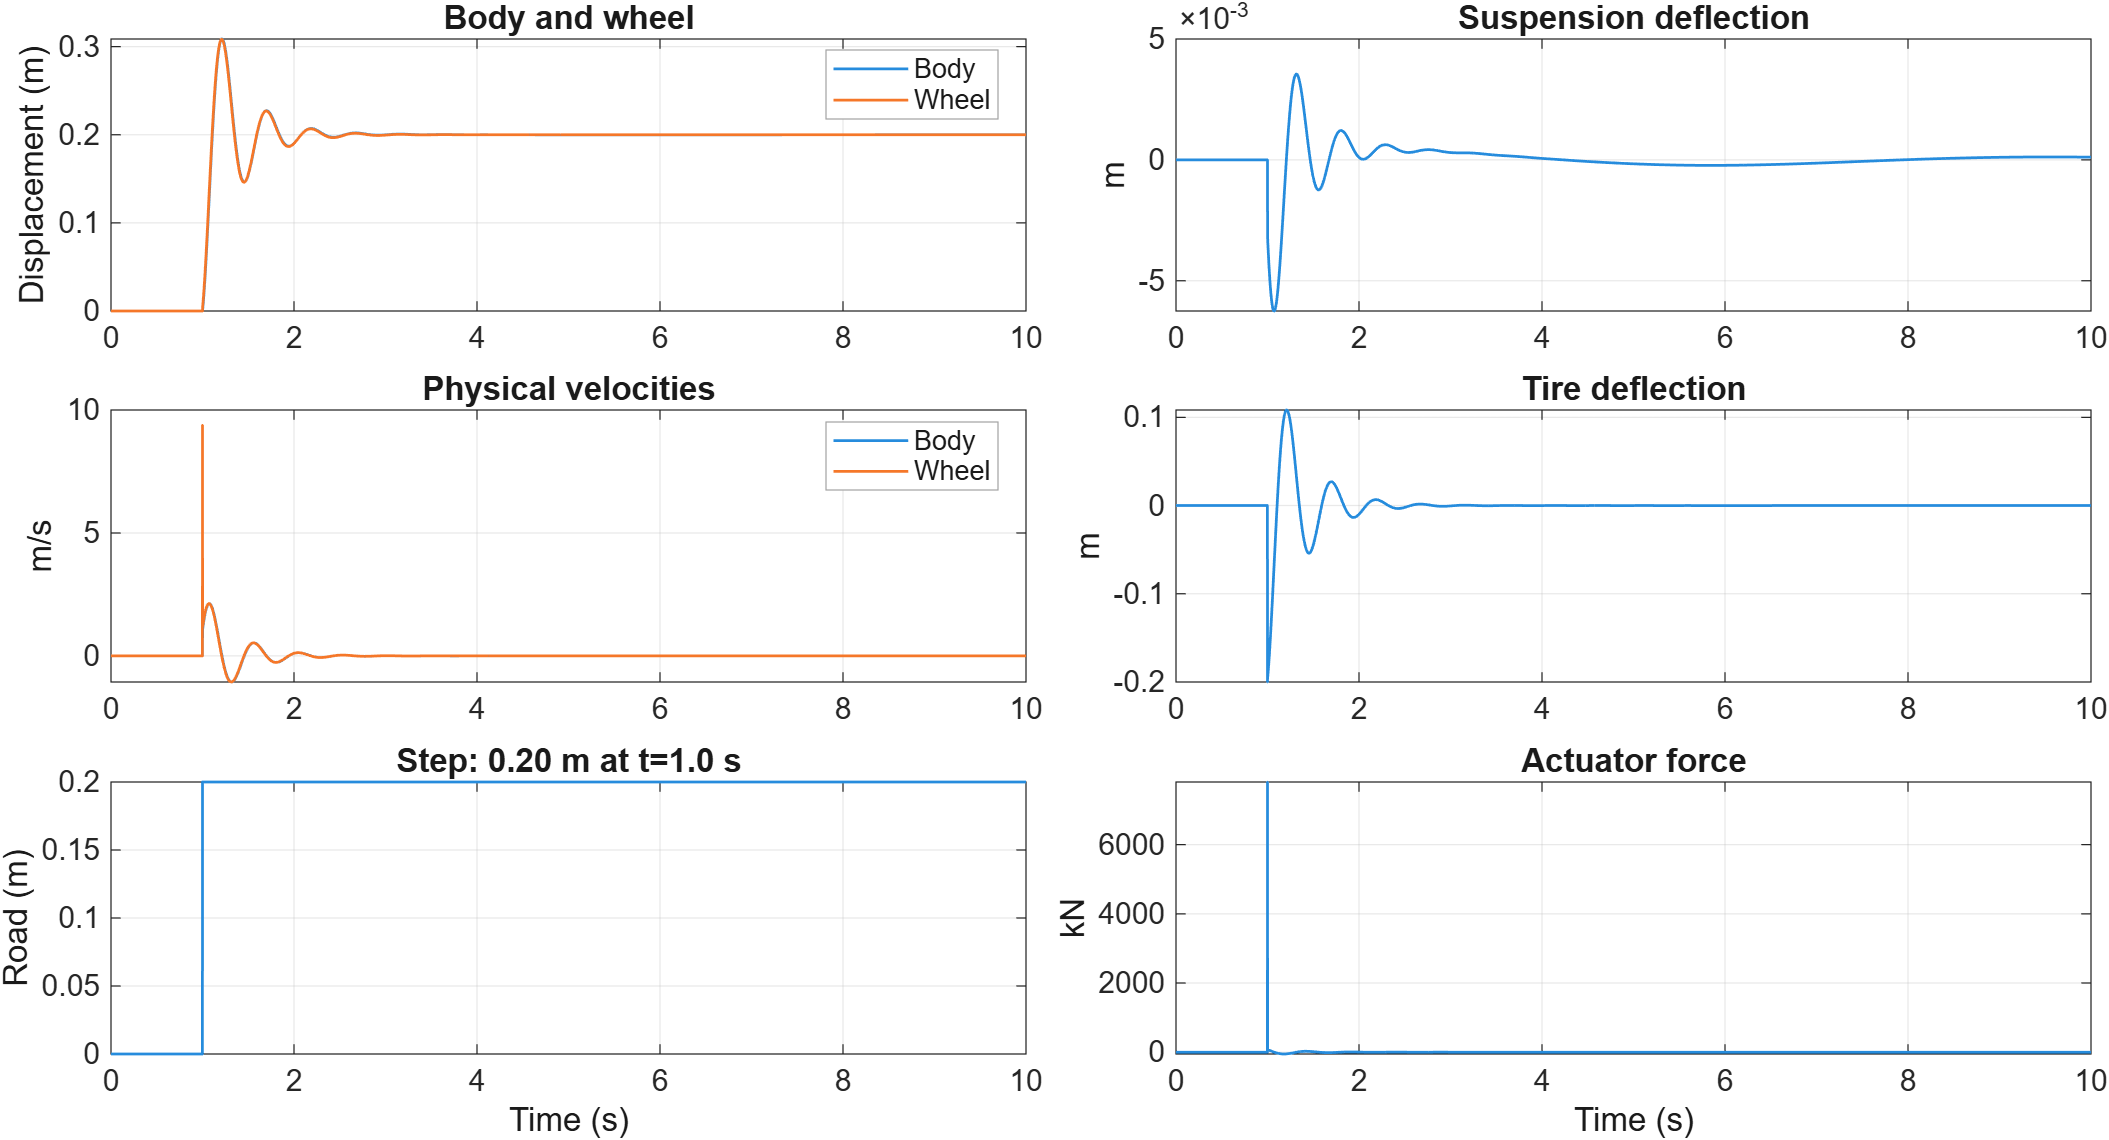
\includegraphics[width=0.88\linewidth]{figures/corrected_pid_step.png}
\caption{PID step response, regenerated in MATLAB using the original six-panel layout.
The force peak is 7810.4 kN; the extreme initial transient is an ideal-model result.}
\end{figure}
\begin{figure}[H]\centering
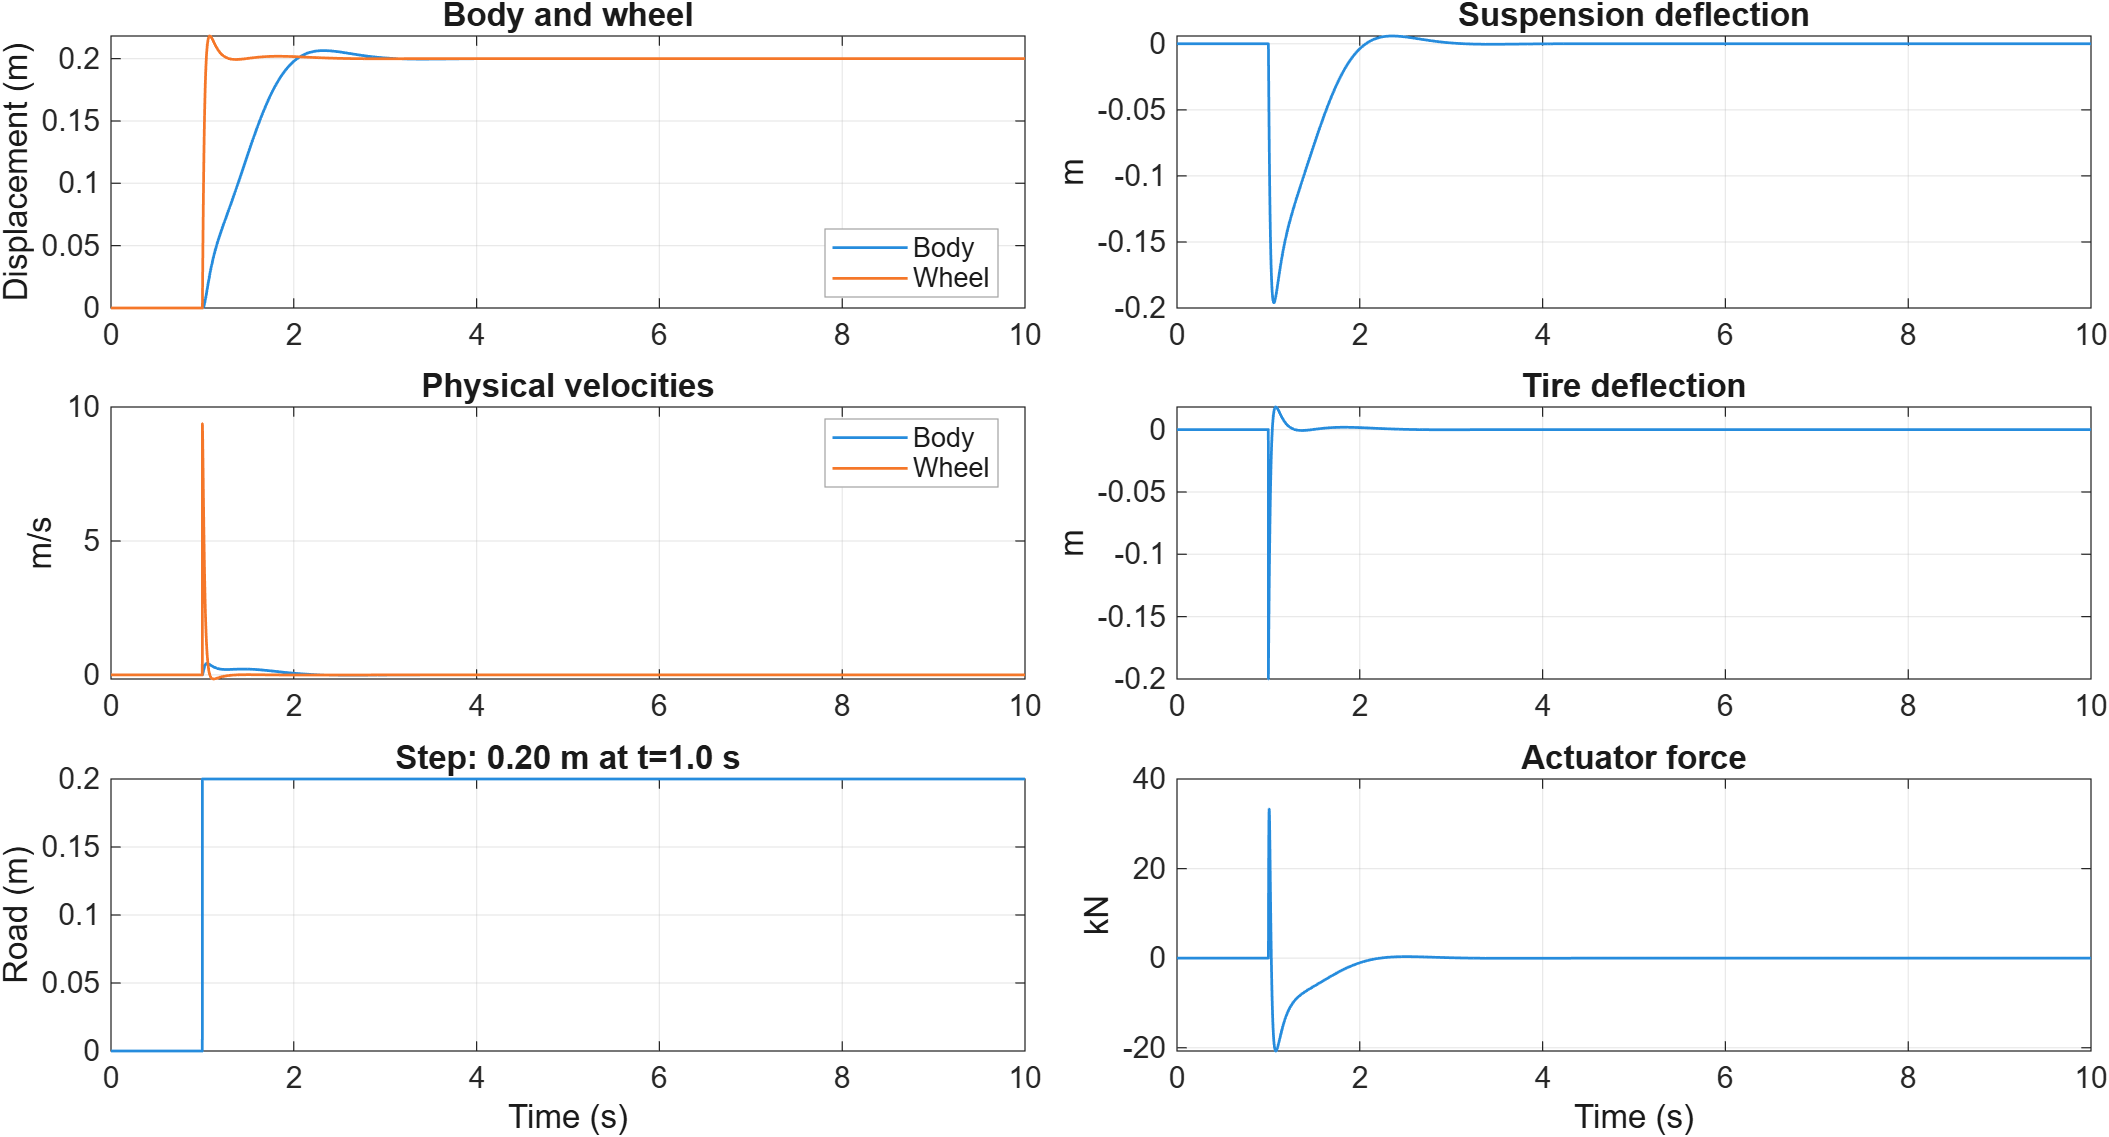
\includegraphics[width=0.88\linewidth]{figures/corrected_lqr_step.png}
\caption{LQR step response with the documented five-state gain and weights.}
\end{figure}
\newpage
\section*{Corrected MATLAB figures: sinusoidal road}
\begin{figure}[H]\centering
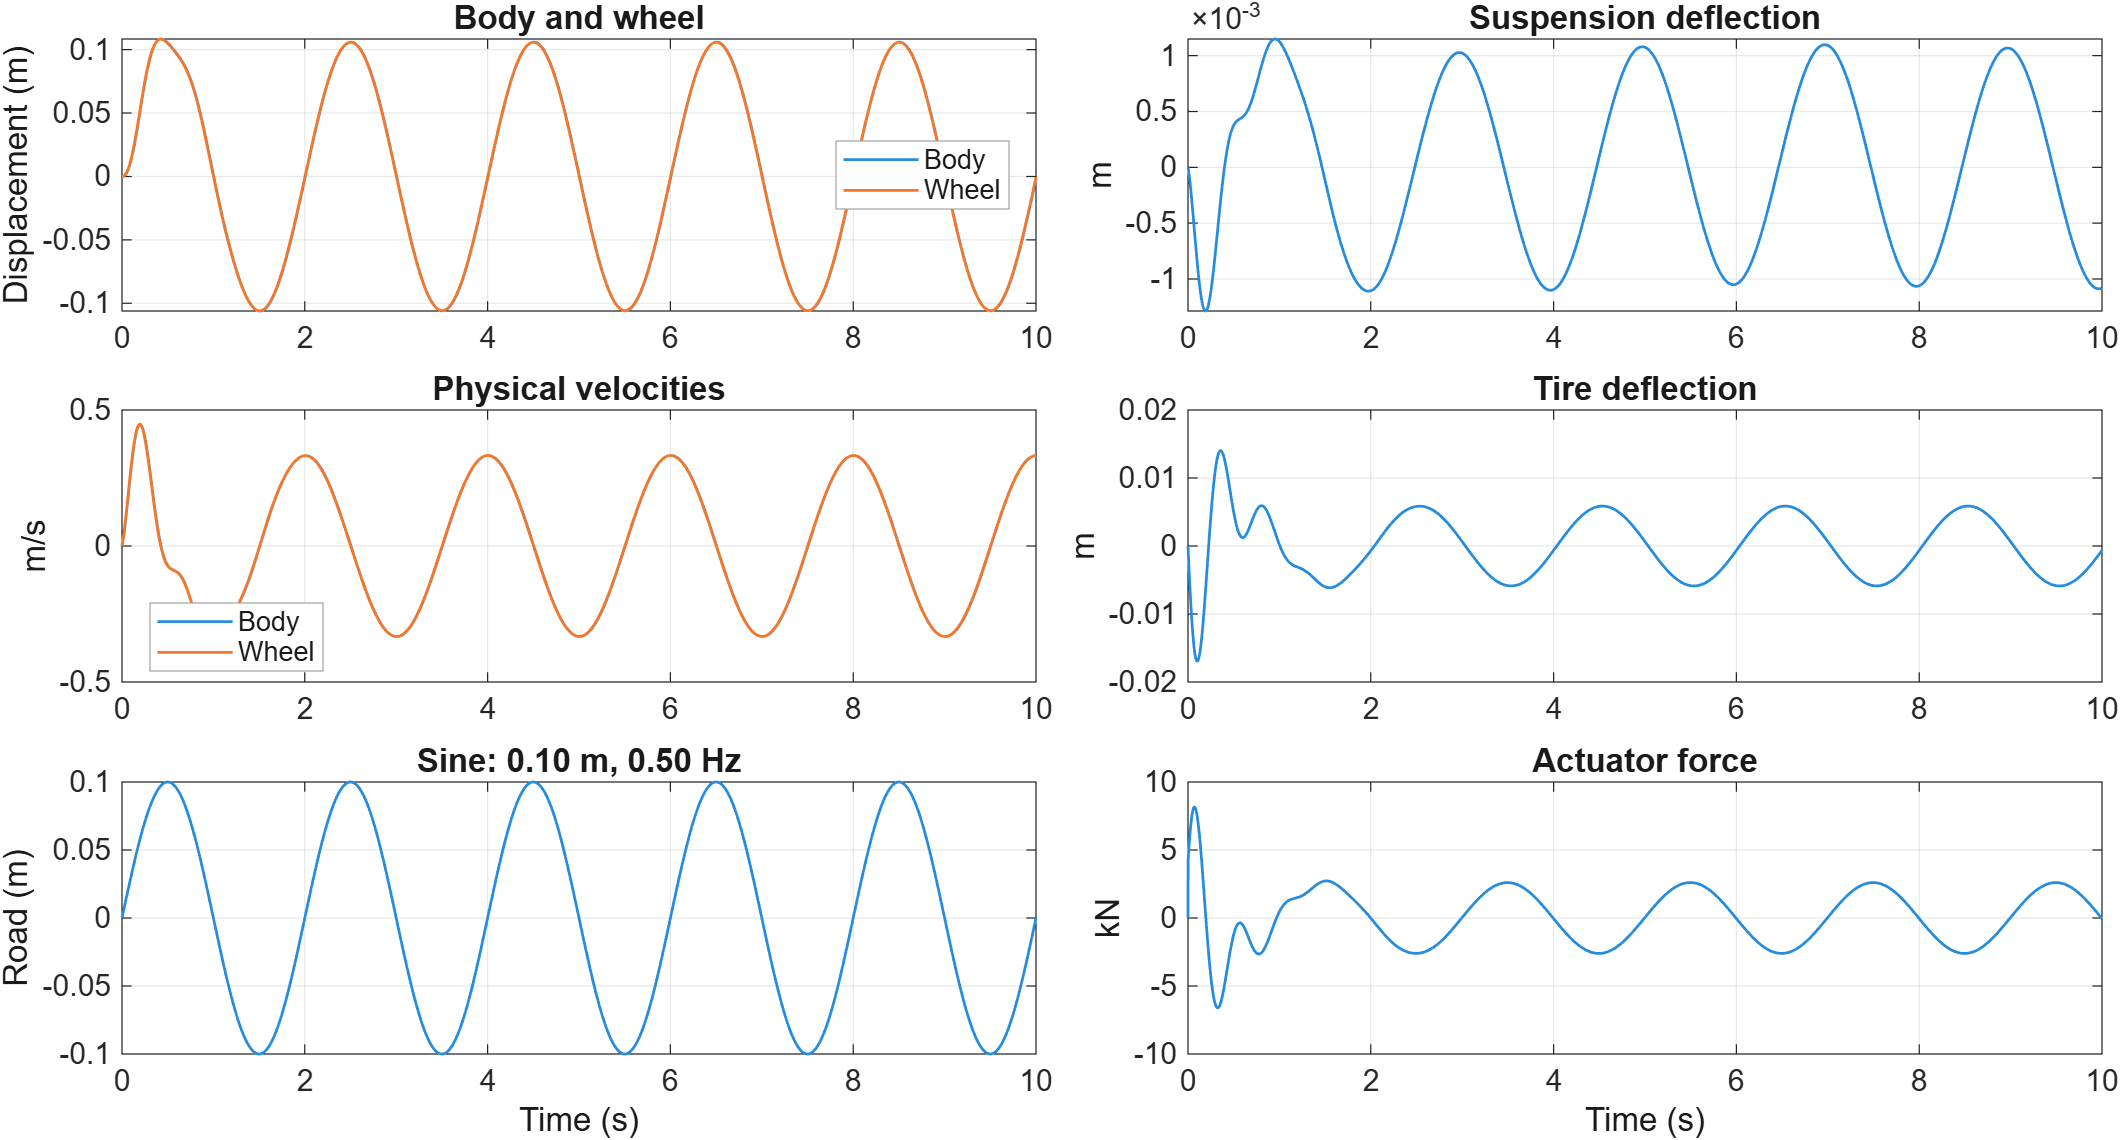
\includegraphics[width=0.88\linewidth]{figures/corrected_pid_sine.png}
\caption{PID response to the 0.10 m, 0.5 Hz sine, including the startup transient.}
\end{figure}
\begin{figure}[H]\centering
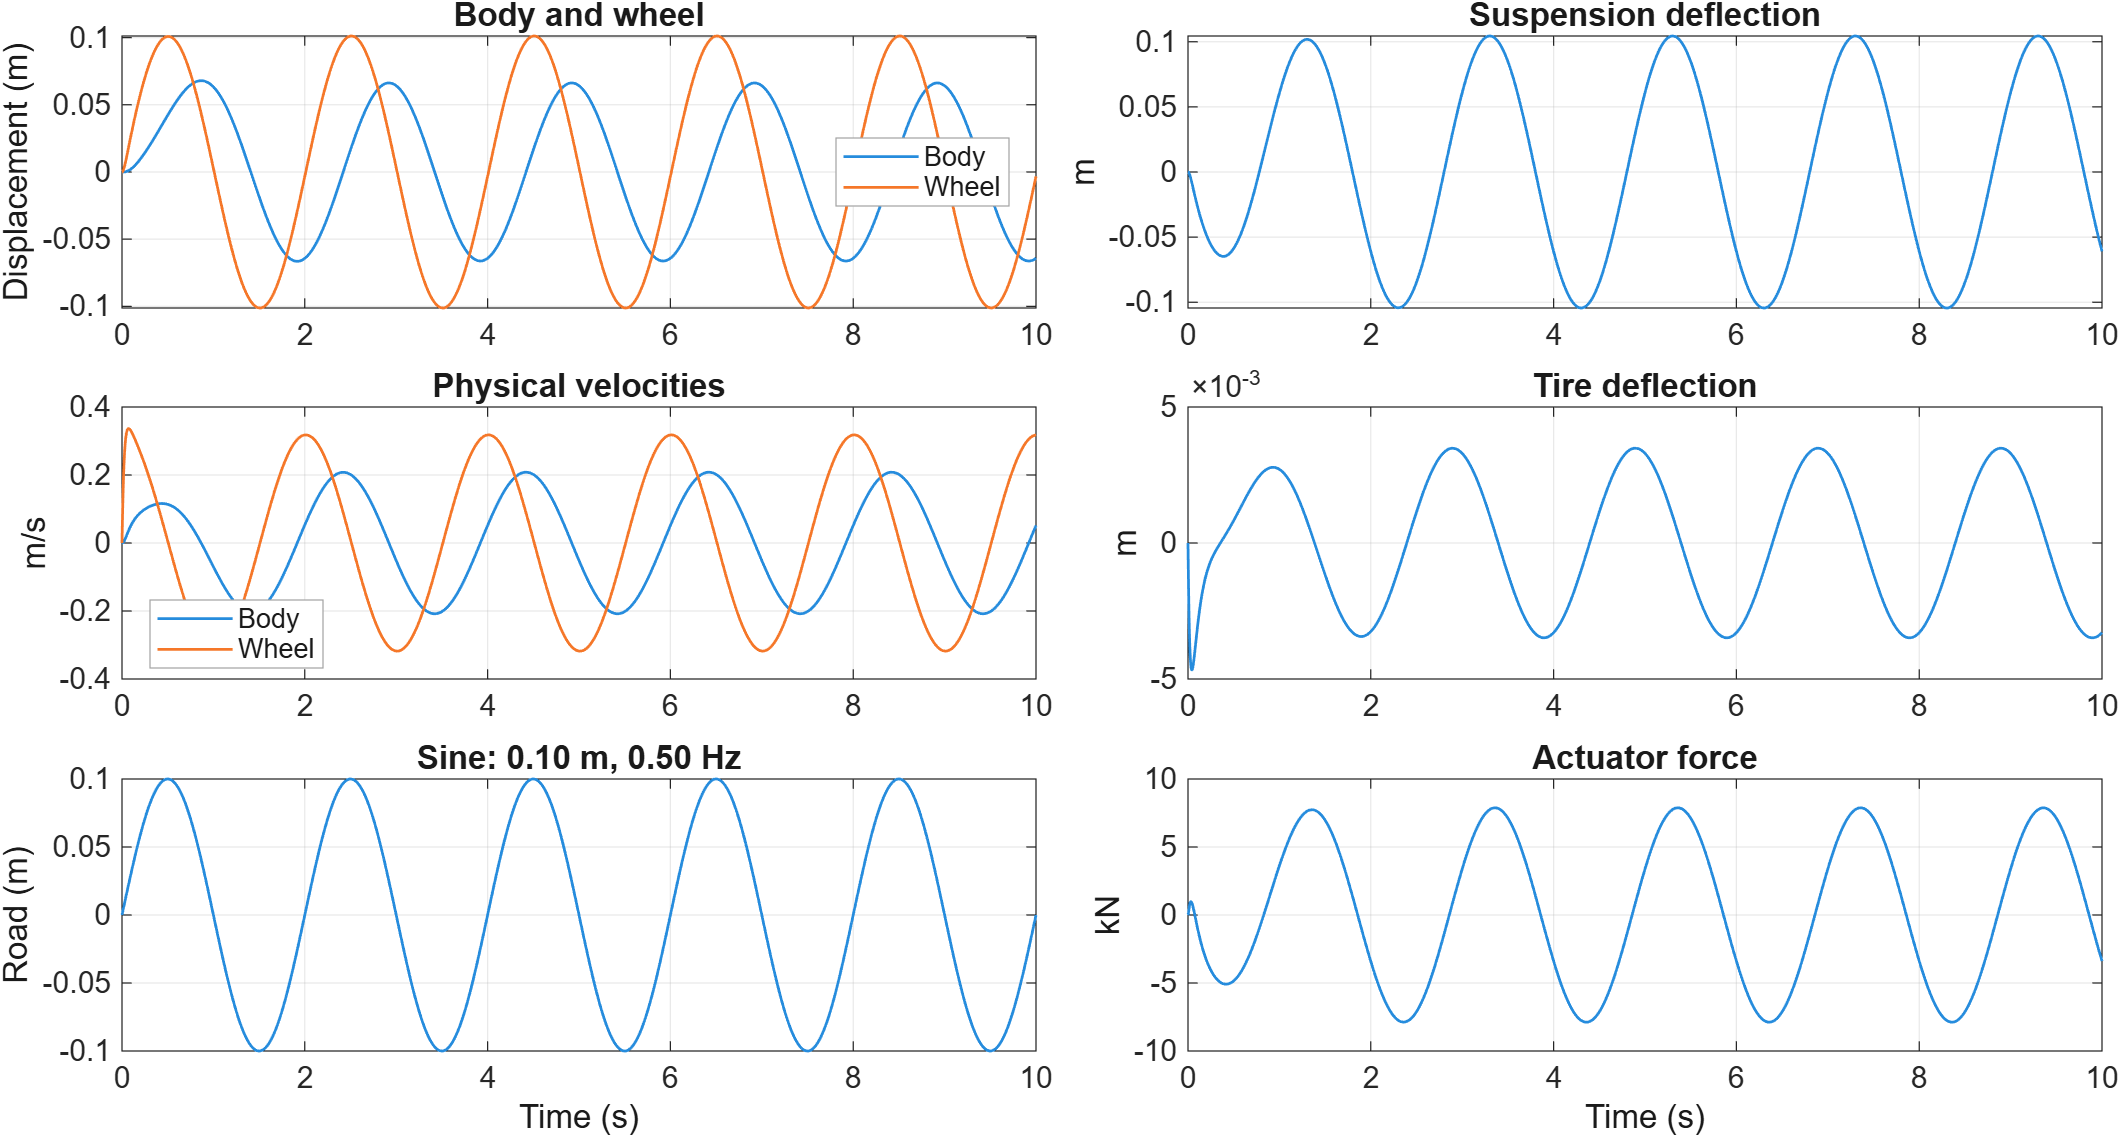
\includegraphics[width=0.88\linewidth]{figures/corrected_lqr_sine.png}
\caption{LQR response to the same sine. Improved comfort comes with substantial travel and force.}
\end{figure}
\newpage
\section*{Passive baseline in MATLAB}
\begin{figure}[H]\centering
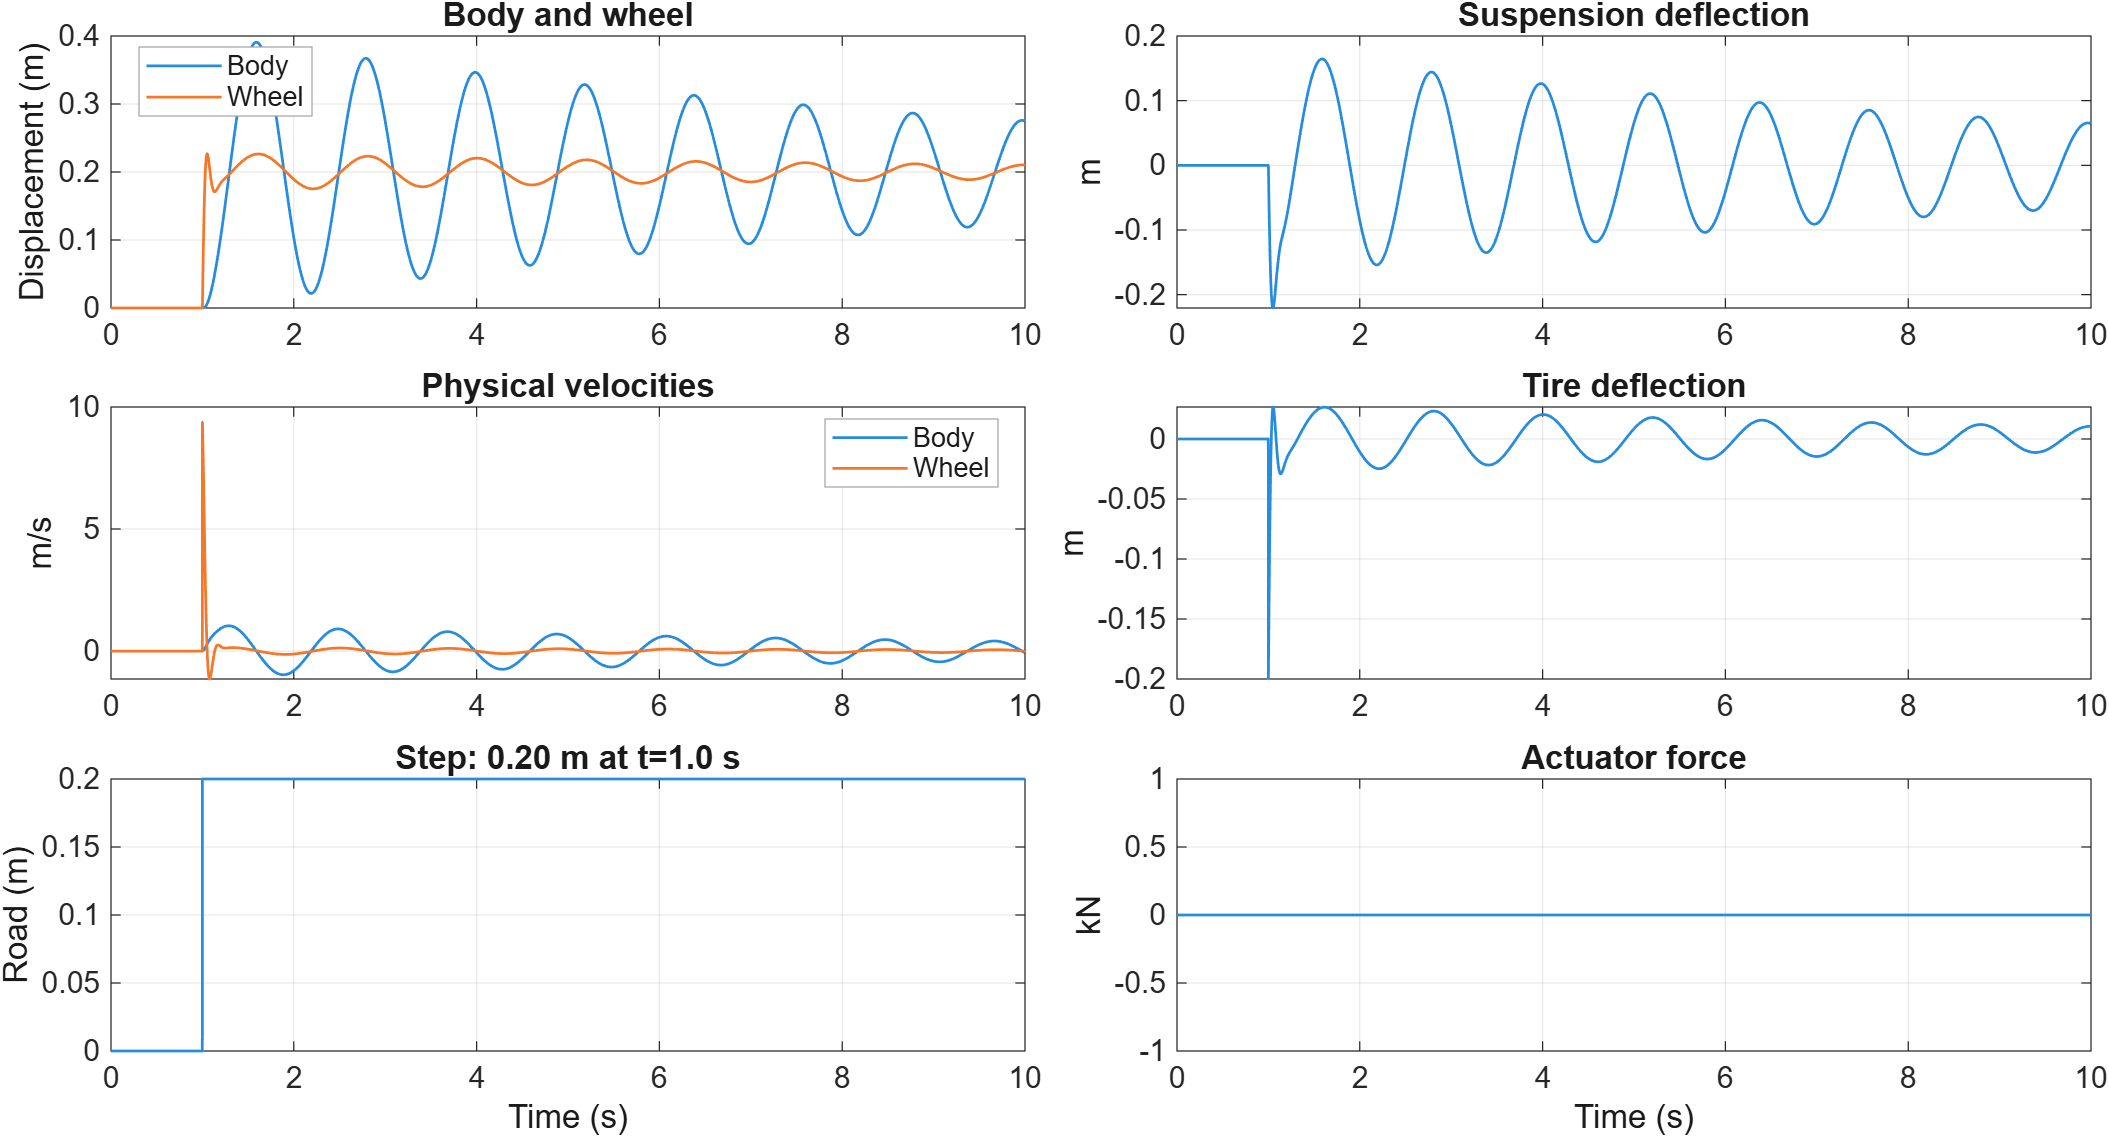
\includegraphics[width=0.88\linewidth]{figures/corrected_passive_step.png}
\caption{Passive response to the road step. Slow body-mode decay persists beyond the record.}
\end{figure}
\begin{figure}[H]\centering
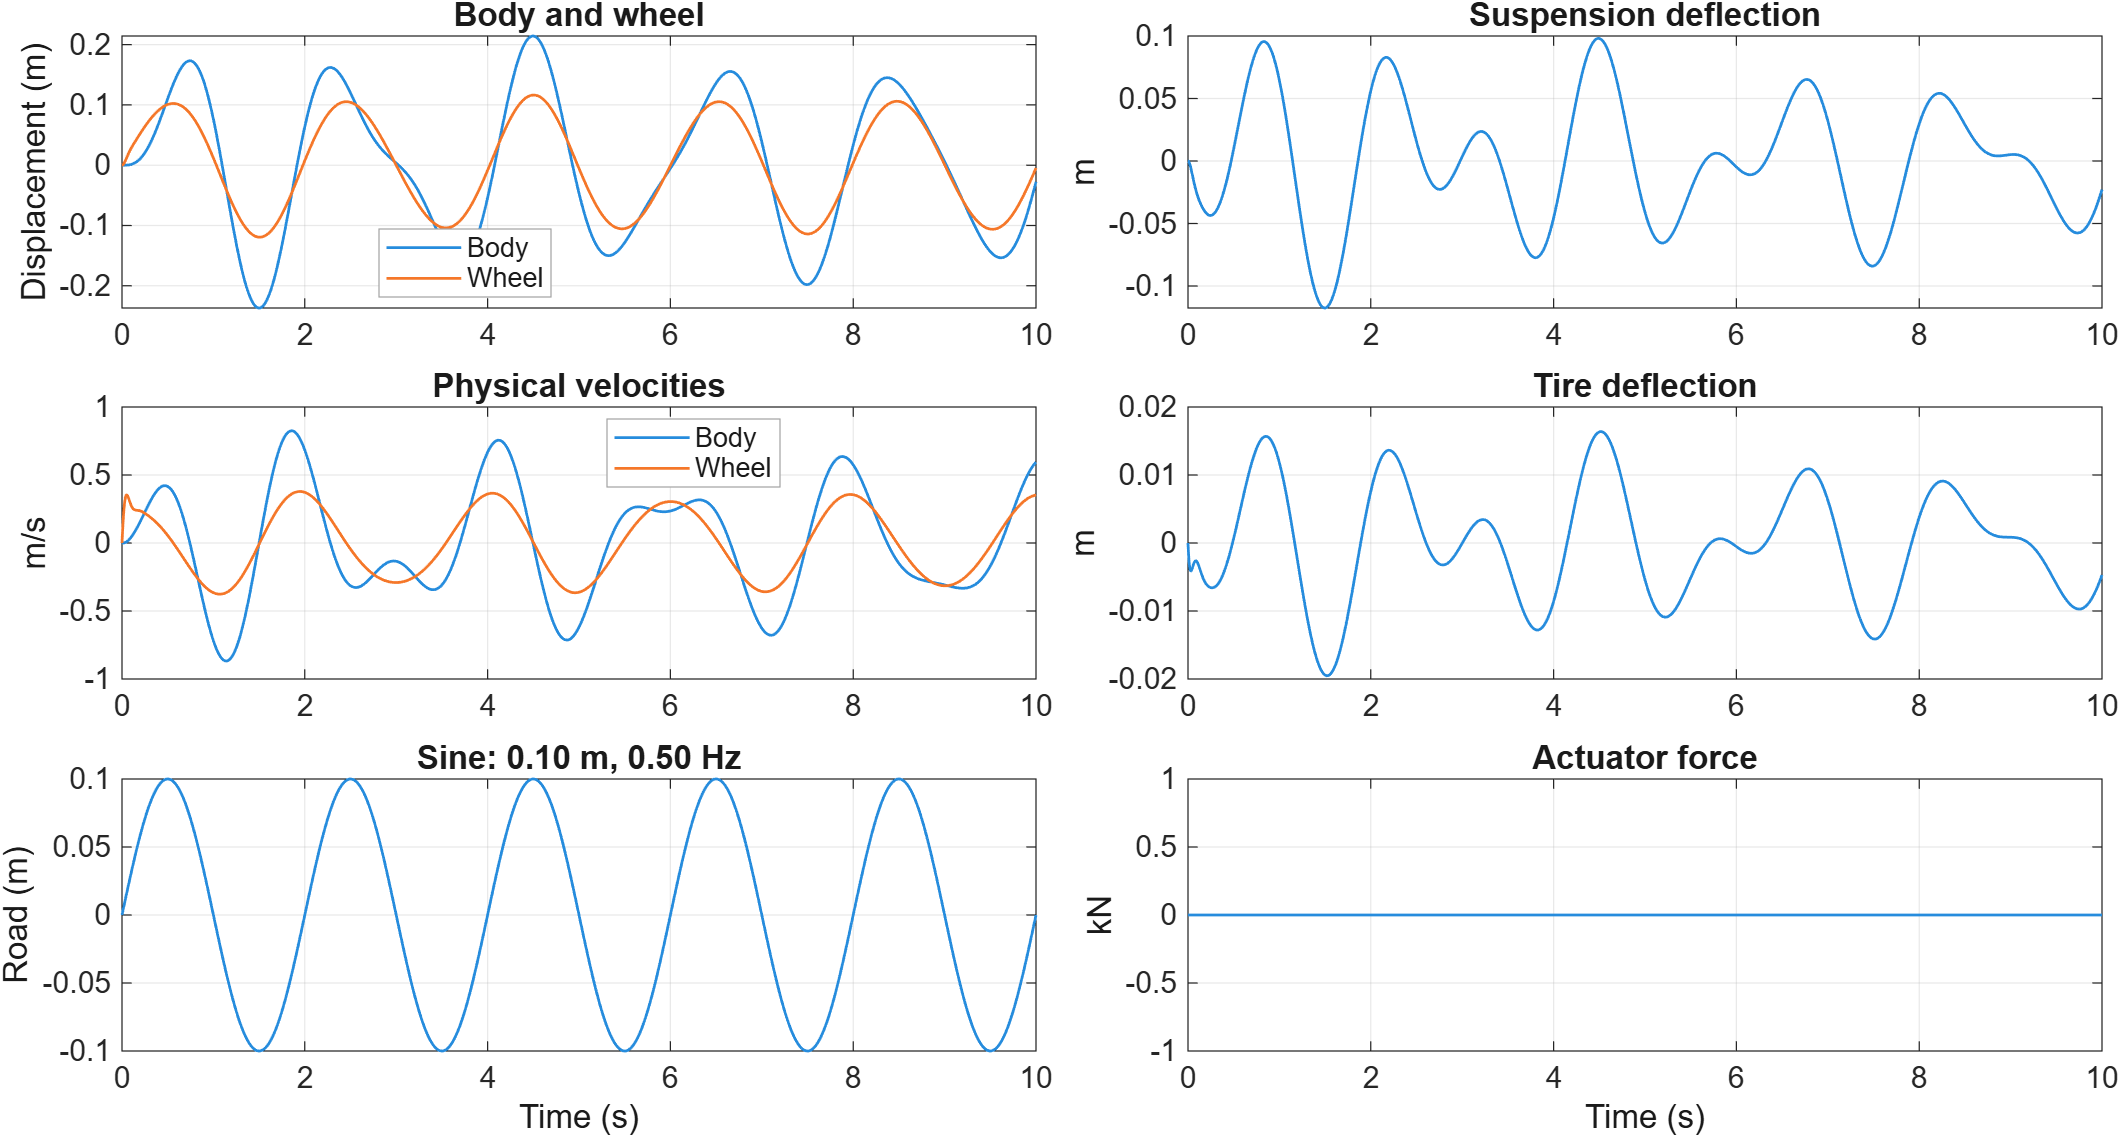
\includegraphics[width=0.88\linewidth]{figures/corrected_passive_sine.png}
\caption{Passive sine response used as the common baseline for both controllers.}
\end{figure}
\newpage
\task{Task 3(a): Comfort and road-holding tradeoffs}
In the step case LQR reduces acceleration RMS from 2.498 to 0.753 m/s$^2$ and
tire RMS from 0.01364 to 0.00613 m relative to passive operation. However, peak
travel remains about 0.196 m. The PID's 0.00625 m peak travel looks attractive
in isolation, but its 13.275 m/s$^2$ acceleration RMS and enormous force spike
show the price of tying body motion tightly to the wheel. In the sine case,
LQR reduces both acceleration and tire RMS more than this PID tuning, while
allowing about 0.104 m peak travel and using 5.384 kN RMS force. No controller
dominates all metrics. Tire deflection is only a proxy: contact requires examining
normal force and a model that permits tire separation.
\task{Task 3(b): Practical actuator and implementation limits}
The ideal PID step peak is about 7.81 MN, compared with the LQR peak of 33.3 kN.
Neither value should be accepted as a hardware requirement without a realistic
road transition and actuator model. Required stroke must accommodate suspension
travel, and speed must accommodate $\dot x_s$. The actuator's mechanical power is
$P_{\mathrm{mech}}=u(\dot z_s-\dot z_u)=u\dot x_s$, not $u^2$; electrical energy
also depends on losses and regeneration. RMS force is useful for effort comparison
but is not an energy estimate.

Replace ideal derivative action with, for example,
\begin{equation}
 C_{\mathrm{PID},f}(p)=K_p+K_i/p+\frac{K_dp}{1+\tau_fp},\qquad \tau_f>0.
\end{equation}
Introduce the filter state, retune, and recheck poles and disturbance responses.
Add force/rate saturation and anti-windup. Integral-augmented LQR also needs
anti-windup if the actuator saturates; its optimality and linear stability results
do not automatically carry over to saturation. An implementation also needs
sensors or an observer for the physical/transformed states; the present solution
assumes full-state availability and known road input where required for reconstruction.
\task{Task 3(c): What can be concluded about robustness?}
For these nominal parameters and two specified roads, LQR provides better comfort
and tire-deflection metrics than the supplied PID, but requires more travel and,
for the sine, more RMS force. This is evidence about nominal performance, not proof
of greater robustness to uncertain mass, damping, sensor noise, or delays.

A defensible next study would hold each gain fixed, vary $M_s$ (for example,
$\pm20\%$) and damping ($\pm20\%$), sweep road frequency, and recompute stability,
RMS, travel, and force. If transformed-state feedback is reconstructed with nominal
parameters, retain that actual estimator/reconstruction rather than giving the
controller exact uncertain states. Add measurement noise, delay, and actuator
limits, and report the worst cases and uncertainty ranges. Those additional tests
are not claimed by the six nominal cases in this solution.
\task{Task 3(d): Data-driven adaptation and preview}
Road-preview sensors could provide feedforward action before a bump arrives.
Gain scheduling could adapt to load and speed; data-driven optimization could
choose validated tuning sets from road statistics. Required data include synchronized
road height, speed, body/wheel motion, forces, and representative loads. Preview
latency, occlusion, unseen roads, sensor faults, and changing tire properties must be
tested. Constrain adaptation to a validated operating region, monitor force/travel,
and retain a stable fallback controller. Prediction quality alone is insufficient
evidence of closed-loop safety or reliability.
\newpage
\appendix
\section*{Appendix A: MATLAB implementation}
The following are the actual executable repository files, included directly with
\texttt{\string\lstinputlisting} to keep the printed code synchronized. They retain
the original MATLAB listing colors, line numbers, light-gray background, and frame.
Run \texttt{quarter\_car\_demo\_solution.m} from MATLAB. Change
\texttt{control\_mode} and \texttt{road\_input} to select a case. The separate
\texttt{animate\_step\_comparison.m} produces controlled/passive overlay animations.
\subsection*{Configuration}
\lstinputlisting[language={},numbers=none]{../solutions/config.json}
\subsection*{Main script: parameters, simulation, plots, and animation}
\lstinputlisting{../solutions/quarter_car_demo_solution.m}
\newpage
\subsection*{Model, PID/LQR control, and exact simulation}
\lstinputlisting{../solutions/simulate_quarter_car.m}
\subsection*{Performance metrics}
\lstinputlisting{../solutions/quarter_car_performance_eval.m}
\section*{Appendix B: Reproduction and checks}
Run \texttt{tools/validate\_matlab.m} for the native six-case checks and
\texttt{tools/export\_document\_figures.m} to regenerate the plots in this PDF.
For independent Python checks and the document build, run:
\begin{lstlisting}[language={},numbers=none]
python tools/build_previews.py
python tools/validate_repository.py
python tools/build_documents.py
\end{lstlisting}
The default LaTeX engine is Tectonic in the Conda environment \texttt{latex-env}.

\end{document}
